
note pour intro :

\begin{itemize}
	
	\item $S^{2n-1}$ est semblable au produit $\U{1}\times \PC{n-1}$ mais que de façon local. C'est un exemple de variété fibré et de ce formalisme donc on aura besoin
	
	\item Aussi, par souci de comodité, on se placera dans $\C^{n+1}$ et l'on notera la sphère unité de ce dernier :
	\[\S{n} \defeq S^{2n+1}\]
	
	\item Tout le formalisme nécessaire sera exposé dans la \cref{sec:cadre_geodiff}, avec plus de détail technique en annexe et dans la \cref{sec:phases_dans_VFP} seront décrites les différentes phases d'un point de vue géométrique.
	
\end{itemize}



\section{Cadre d'étude}\label{sec:cadre_geodiff}

Pour proprement poser le cadre, il nous faudra trois choses :
\begin{enumerate}
	
	\item D'abord faire quelque rappel de géométrie différentielle, ne serait-ce que pour fixer les notations (\Cref{subsec:rappel2geo_diff}), avec comme exemple le cas $\PC{n}$ (\Cref{subsec:PC^n_variet}), qui sera utile plus loin. 
	
	\item Ensuite, seront définies les variétés fibrés principales, avec les outils de bases qui leurs sont associés (\Cref{subsec:def2VFP}), puis $\U{1}\times \PC{n}$ sera écrit comme telle (\Cref{subsec:SUPC_VFP}).
	
	\item Enfin, il nous faudra définir une connexion sur ces fibrés, connexion qui seront, d'abord, définie de façon générale (\Cref{subsec:def2conn}), puis explicitée et interprétée dans le cas qui nous intéresse (\Cref{subsec:conn2SUPC}).
	
\end{enumerate}

\subsection{$\bf{\PC{n}}$ vue comme variété différentielle} \label{subsec:construc_PC^n}

\subsubsection{\wip Rappels de géométrie différentielle et notations}\label{subsec:rappel2geo_diff}

\thoughts{À compléter en fonction du la suite}
\\

Une variété différentielle se définie comme suit :
\begin{definition}[Variété différentielle] \label{defvarietoche}
	une variété différentielle de classe $C^k$ de dimension $n$ est un espace topologique
	$\manu$ munie d'un \emph{atlas} $\big\{ (\phi_i, U_i) \big\}_{i\in I}$, c'est-à-dire un ensemble finie de pair d'ouvert $U_i\subset \manu$ et d'application $\phi_i :U_i\ \lr\ \R^n$ telle que :
	\begin{itemize}
		
		\item les $U_i$ forme un recouvrement de la variété :\qquad $\bigcup_{i\in I} U_i = \manu$
		
		\item les $\phi_i$ sont des homéomorphismes sur leur image $\phi_i(U_i)\subset\R^n$.
		
		\item si l'intersection $U_i \cap U_j$ est non vide, alors ${\phi_j \circ {\phi_i}^{-1}}_{| {\phi_i}(U_i\cap U_j)}$ est un $C^k$ difféomorphisme sur son image.
		
	\end{itemize}
	A travers $\phi_i$, à tout point $x\in U_i$ sont associées des \emph{coordonnées locales} $(x^\mu)_{1\leq \mu\leq n}$, c'est-à-dire les coefficient de $\phi_i(x)$ dans une base $(e_\mu)_{1\leq \mu\leq n}$ de $\R^n$. Ces coordonnées sont dites locales car dépendantes du choix de la pair $(U_i,\phi_i)$ et la composée ${\phi_j \circ {\phi_i}^{-1}}_{| {\phi_i}(U_i\cap U_j)}$ est vue comme un \emph{changement de coordonnées}.\\
	Dans toutes la suite, toutes les objets propre au cartes seront indexes via l'alphabet classique ($i,j,k$) et le indices associées au coordonnées locales par des lettres grecs ($\mu,\nu,\alpha$).
\end{definition}

\begin{figure}[h]
	
\includegraphics[width=0.6\textwidth]{fig/placeholder}
	\caption[La première figure de tout bon livre de géométrie différentielle]{La première figure de tout bon livre de géométrie différentielle : représentation de deux cartes avec l'application de changement de coordonnées}
\end{figure}

Ensuite, les \emph{espaces tangents} de $\manu$  et son fibré tangent seront respectivement notés :
\begin{align}
	\forall x\in\manu,\ &\tg[x]{\manu}  &  \tg{\manu} &= \bigsqcup_{x\in\manu}\tg[x]{\manu}
\end{align} 
Pour le dire rapidement, les vecteurs tangents agissent comme une dérivation en cela que, pour une chemin $\gamma : \R\lr\manu$, sa différentielle au point $x=\gamma(0)$ est définie par l'application :
\begin{equation} \label{eq:def2vec_tg}
	\dot{\gamma}_{x}\  :\ \begin{aligned}
		\conti[1]{\manu}{\R}\ &\lr\qquad \R \\ 
		f\qquad &\lmt\ \frac{d}{dt} f \circ\gamma(t)\Big|_{t=0} \defeq \frac{d(f \circ \gamma)}{dt}(0)
	\end{aligned}
\end{equation}
\\
Aussi, le système de coordonnées locales en $x\in\manu$ induit une base sur $\tg[x]{\manu}$, qui sera noté  $\bt_\mu = \frac{\partial}{\partial x^\mu}$. notation qui est justifié en cela que, moralement, $\bt_\mu$ dérive toute fonction test $f\in\conti[k]{\manu}{\R}$ dans le long de la $\mu^{eme}$ coordonnée (locale) de $x$.
\\

Plus généralement, si $\manu$ et $\mathpzc{N}$ sont deux variétés différentielles et $f : \manu\lr \mathpzc{N}$ une application différentiable avec $\{\Tilde{\bt}_\nu\}_\nu$ une base de $\tg{\mathpzc{N}}$, sa différentielle (ou application tangent ou push forward) au point $x$ est l'application linéaire qui, en coordonnée local s'écrit :
\[f_*(\bf{v}) = f_*(v^\mu \bt_\mu) = \bt_\mu\big( f^\nu \big)v^\mu \Tilde{\bt}_\nu\qquad \text{ ou encore }\qquad  (f_*)_\mu^\nu = \bt_\mu\big( f^\nu \big)\]
\\
A partir de  $f_*$ est définie l'image réciproque ou pull back de $f$, qui correspond moralement à la transposée de $f_*$. Formellement elle est définie par dualité :

\[f^*\ :\ \begin{aligned}
	\tg{^*\mathpzc{N}}\ &\lr\ \tg{^*\manu} \\ g\quad\ &\lmt\ g\circ f^*
\end{aligned} \]


\begin{figure}[h]
	\begin{tikzcd}[column sep=large]
		\manu \arrow[d]  \arrow[r, "f" above]  & \mathpzc{N} \arrow[d]\\
		\tg{\manu} \arrow[d]  \arrow[r, "f_*" above]  & \tg{\mathpzc{N}} \arrow[d]\\
		\tg{^*\manu}  & \tg{^*\mathpzc{N}} \arrow[l, "f^*" above]
	\end{tikzcd}
	\caption{Diagramme commutatif du passage de $f$ à sa différentielle et/ou à son image réciproque}
	\label{fig:diagc_pullb/pushf}
\end{figure}

\begin{itemize}
	
	\item fibré tangent dual
	
	\item image réciproque (``transposé'' de la différentielle)
	
	\item métrique riemannienne
	
\end{itemize}



\subsubsection{\wip $\bf{\PC{n}}$ comme variété différentielle} \label{subsec:PC^n_variet}


Si l'espace projectif complexe à été présenté comme le quotient $\S{n}/\U{1}$, il peut aussi être vu comme :
\[\PC{n} \cong {\C^{n+1}}^*/\C^*\]
C'est-à-dire l'ensemble des classes de ${\C^{n+1}}^* = \C^{n+1} \setminus \{0_{\C^{n+1}}\}$ par la relation d'équivalence :
\[x \sim y\ \Llr\ \exists \lambda\in\C^*\ |\ x=\lambda y\]
\\
Moralement, en isolant la norme des vecteurs, ${\C^{n+1}}^*$ peut être vu comme le produit $\R^{+_*} \times \S{n}$, et de même pour $\C^*$ avec le module :
\begin{align*}
	{\C^{n+1}}^* &\cong \R^{+_*} \times \S{n}  &  \C^* &\cong \R^{+_*} \times \U{1}
\end{align*}
\\
Ainsi, le quotient par $\C^*$ revient à regarder les vecteurs de ${\C^{n+1}}^*$ modulo leur norme, puis modulo l'action de $\U{1}$. Or, ignorer la norme des vecteurs est équivalent à ne regarder que les vecteurs normées, donc les vecteurs de $\S{n}$. De façon informelle, on pourrait alors écrire\footnote{\itshape
	Ce qui s'écrit plus justement avec le troisième théorème d'isomorphisme : \[{\C^{n+1}}^*/\C^* \cong ({\C^{n+1}}^* / \R^{+_*})/(\C^* / \R^{+_*}) \cong \S{n}/\U{1} = \PC{n}\]
} :
\begin{align*}
	{\C^{n+1}}^*/\C^* &\cong {\C^{n+1}}^*/(\R^* \times \U{1})\\
	&\cong \big( {\C^{n+1}}^*/\R^* \big) /\U{1} \\
	&\cong \S{n}  / \U{1} = \PC{n} 
\end{align*}
\skipl

L'intérêt de cette écriture et que $\C^{n+1}$ est un espace vectoriel, ce qui permet de décrire $\PC{n}$ en terme de carte, ce qui se fait comme suit.
La classe de $\PC{n}$ de représentant $z = (z^i)_{0\leq i\leq n}\in{\C^{n+1}}^*$ est noté $[z]$ et on pose, $\forall i\in\llbracket0,n\rrbracket$ :
\begin{align}
	U_i &= \Big\{[z]\in\PC{n}\ \big|\ z\in \C^{n+1},\ z^i\neq 0\Big\}  &  \phi_i\  :\quad &\begin{aligned}
		U_i\ \ &\lr\quad\ \C^{i}\times \{1\} \times\C^{n-i}\cong \C^{n} \\ [z]\ \ &\lmt\ \frac{1}{z^i}z = \big(\nicefrac{z^0}{z^i},\cdots, 1, \cdots, \nicefrac{z^n}{z^i}\big)
	\end{aligned}
\end{align}
\begin{remarque}
	Si l'ensemble d'arrivé $\phi_i(U_i)$ est équivalent à un ouvert de $\C^{n}$ (l'une des composantes est constante), il est plus commode de travailler dans $\C^{n+1}$ puisque cela évite de devoir enlever et rajouter des coefficient dans les formules de changement de carte :
	\[ \forall z\in\C^{n+1}\ |\ z^{i,j}\neq 0\quad (\ie~[z]\in U_i\cap U_j) ,\qquad \phi_i \circ {\phi_j}^{-1}(z) = \frac{z^j}{z^i}z\]
\end{remarque}
\skipl
Les $(U_i,\phi_i)$ forment un atlas sur l'espace projectif complexe, faisant de ce dernier une variété de dimension $\dim = 2n$. Les $\phi_i \circ {\phi_j}^{-1}$ étant holomorphe, $\PC{n}$ est plus précisément une variété complexe de dimension complexe $n$ et il est utile d'écrire ses coordonnées locales sous la forme $(w^\mu, \congu{w}^\mu)_{1\leq \mu \leq n}$, où :
\[\forall w\in U_i,\ \forall \mu\neq i,\quad w^\mu = \frac{z^\mu}{z^i},\qquad  \text{ où }\quad [z] = w\]
\\
En annexe \ref{ann:VDC} se trouve plus de détail sur les variétés différentielles complexes, mais pour aller à l'essentiel, mais si la notation prête à confusion, il faut considérer les coordonnées $w^\mu$ et $\congu{w}^\mu$ comme complètement décorréler. Par exemple, :
\begin{align*}
	\bt_\mu(w^\mu) &= \frac{\partial}{\partial w^\mu} w^\mu = 1  &  
	\bt_{\congu{\mu}}(w^\mu) = \frac{\partial}{\partial \congu{w}^\mu} w^\mu &= 0 
		\\
	\bt_\mu(\congu{w}^\mu) &= \frac{\partial}{\partial w^\mu} \congu{w}^\mu = 0  &  
	\bt_{\congu{\mu}}(\congu{w}^\mu) = \frac{\partial}{\partial \congu{w}^\mu} \congu{w}^\mu &= 1
\end{align*}
Ce qui fait $(w^\mu, \congu{w}^\mu)_{1\leq \mu \leq n}$ est bien une base de dimension réelle $\ \dim[\R]\PC{n} = 2n$. Ces ``notations'' (encore une fois \cf~annexe \ref{ann:VDC}) permettent, par exemple, de décrire le fait qu'une soit fonction holomorphe $f: \PC{n}\lr \C$ par la contrainte :
\[\forall w\in\PC{n},\ \forall \mu,\qquad \frac{\partial}{\partial \congu{w}^\mu}f(w) = 0\] 
\\
Pour ce qui est des espaces tangents, $(\bt_\mu, \bt_{\congu{\mu}})_\mu$ forme une base de $\tg{\PC{n}}$ et $(dw^\mu, d\congu{w}^\mu)_\mu$ une base de $\tg{^* \PC{n}}$.
\\
$\PC{n}$, en particulier, admet un produit hermitien plus connue sous le nom de métrique de Fubini-Study, donné par :
\begin{equation}
	\begin{aligned}
		\forall w\in\PC{n}, \forall \bf{u},\bf{v}\in\tg[w]{\PC{n}},\qquad g_w(\bf{u}, \bf{v}) = g_{\mu\congu{\nu}} u^\mu \congu{v^\nu} 
		&= \frac{(1+w^\alpha \congu{w}_\alpha)\delta_{\mu\nu} - w_\mu \congu{w}_\nu}{(1+w^\alpha \congu{w}_\alpha)^2}u^\mu \congu{v}^\nu \\
		&= \frac{1}{1+w^\alpha \congu{w}_\alpha} u^\mu \congu{v}_\mu - \frac{w_\mu \congu{w}_\nu}{(1+w^\alpha \congu{w}_\alpha)^2} u^\mu \congu{v}^\nu
	\end{aligned}
\end{equation}
À noter que seul les coefficients $g_{\mu \congu{\nu}}$ apparaissent. Cela est du au fait que $g$ est produit hermitien, ce qui impose $\ g_{\mu\nu} = 0\ $ et $\ g_{\congu{\mu} \nu} = g_{\mu \congu{\nu}}$.





\subsection{$\bf{S^{2n+1}}$ comme fibré principal} \label{subsec:VFP}

\subsubsection{Définition générale}\label{subsec:def2VFP}

Pour le dire simplement, les \emph{variétés fibrés} sont des variétés qui ressemble localement à des espaces produits. 
Le ruban de Modiüs en est un exemple typique : il ne peut pas s'écrire comme le produit d'un cercle avec un segment $S^{1}\times [0,1]$ à cause de la façon dont il est construit. Mais localement, une tranche du ruban est tout à fait comparable (\ie~difféomorphe) à un tel produit (\cf~\cref{fig:ruban2modius}).
\begin{figure}[h]
	\begin{tikzpicture}[scale=0.8]
	%\draw[opacity=0.1] (-4.5,-4.5) grid (12.5,4.5);
	
	
%%%%     MOBIUS     %%%%

	%main points
	\coordinate (s1-) at ($(90+0-30:4) + (0,-1)$);
	\coordinate (s1+) at ($(90+0+30:4) + (0,-1)$);
	
	\coordinate (s2+) at ($(90+120-30:4) + (0,-1)$);
	\coordinate (s2-) at ($(90-120+30:4) + (0,-1)$);
	
	\coordinate (s3+) at (90+120+30:4);
	\coordinate (s3-) at (90-120-30:4);
	
	%\draw (s1-) -- (s2+) -- (s3-) -- (s1-);
	%\draw (s1+) -- (s3+) -- (s2-) -- (s1+);
	%\draw (s3+) -- (s3-);
	\colorlet{tmpb}{blue!30!};
	\colorlet{tmpr}{red!30!};
	\colorlet{tmpv}{blue!30!red!30!};
	\definecolor{tmpg}{gray}{0.75};
	
	
	% bande droite
	\draw[fill=tmpr] (s1-) .. controls  ($(s1-)+(-60:3)$) and  ($(s3+)+(0:3)$) .. 
		(s3+) -- (s3-) 
		.. controls ($(s3-)+(0:1)$) and ($(s2-)+(-60:1)$) .. 
		(s2-) -- cycle;
		
	% bande haut
	\draw[fill=tmpv] (s1-) .. controls  ($(s1-)+(120:0.5)$) and  ($(s1+)+(60:0.5)$) .. 
		(s1+) -- (s2+) 
		.. controls ($(s2+)+(60:2)$) and ($(s2-)+(120:2)$) .. 
		(s2-) -- cycle;
		
	% bande gauche
	\draw[fill=tmpb] (s1+) .. controls  ($(s1+)+(-120:3)$) and  	($(s3-)+(-180:3)$) .. 
		(s3-) -- (s3+) 
		.. controls ($(s3+)+(-180:1)$) and ($(s2+)+(-120:1)$) .. 
		(s2+) -- cycle;
		
		
	%%%%     CARTE LOCALE     %%%%
	
	% ouvert U_i
	\draw (-1,0.25) -- (-1.5,2.67) node[midway, above right]{$U_i$};
	\draw (1,0.25) -- (1.5,2.67);
	
	% carte
	\draw[fill=tmpg, shift={(6.25,-1.5)}] (0,0) -- (0, 4) node[midway, left]{$G$} -- (3.5,4) -- (3.5,0) -- cycle node[midway, below]{$\pi(U_i)$};
	
	% fleche vers la carte
	\draw[-Stealth, thick] (0,2.5) ..
	controls ($(0,2.5) + (30:2)$)  and ($(7, 2) + (180-30:2)$) .. (7, 2) node[midway, above]{$h_i$};
	
\end{tikzpicture}
	%
\includegraphics[width=0.4\textwidth]{fig/placeholder}
	\caption[Ruban de Mobius comme variété fibrée]{Représentation du ruban de Modius en tant que fibré. Les notations sont reprises de la \cref{def:VFP}.}
	\label{fig:ruban2modius}
\end{figure}
\skipl

Il existe toutes sorte de variétés fibrées dès lors qu'elles sont munies de structure remarquable. Celles qui vont nous intéresser sont dites principales\footnote{\itshape
	Bien que ce ne sera pas précisé, il sera toujours sous-entendu que les différentes variétés et cartes doivent avoir les mêmes niveaux de régularités pour que le tout reste cohérent.} :
\\
\begin{definition}[Variété fibrée principale] \label{def:VFP}
	Une \emph{variété fibrée principale} (VFP), ou \emph{fibré principal} est constituée de deux variétés différentielles $P$ et $B$ telles que :
	\begin{itemize}
		\item Il existe un groupe de Lie $G$ opérant à droite (ou à gauche) sur $P$ via l'application différentiable :
		\begin{equation} \label{eq:VFP_action}
			R\ :\ \begin{aligned}P\times G\ &\lr\quad\ \ P \\ (p,g)\ \ &\lmt\ R_g(p)\defeq p\cdot g = pg
			\end{aligned}
		\end{equation}
		
		\item Il existe une surjection différentiable $\ \pi:P\lr B\ $ telle que :
		\begin{equation} \label{eq:VFP_fibres}
			\forall p\in P,\quad \pi^{-1}\big(\pi(p)\big)=pG
		\end{equation}
		
		\item $P$ est munie d'un ensemble de paire $(U_i, h_i)$ tel que les $U_i$ forment un recouvrement de $B$ et tel que les $h_i : G\times U_i\lr \pi^{-1}(U_i)\subset P$ soient des difféomorphismes vérifiant :
		\begin{align*} \label{eq:VFP_atlas}
			\forall a,b\in G,\ \forall x\in B,\qquad h_i(ab,x) = h_i(a,x) \cdot b\qquad \text{et} \qquad \pi\circ h_i(a,x) = x
		\end{align*}
	\end{itemize}
	
	\begin{adjustbox}{valign=C,raise=1cm, minipage={1.1\linewidth}}
		\begin{wrapfigure}{r}{0.35\textwidth}
			\begin{tikzcd}[column sep=large]
				G\times U_i \arrow[d, "\pr{2}" left]  \arrow[r, "h" above]  & \pi^{-1}(U_i) \subset P \arrow[ld, "\pi" below right] \\
				U_i
			\end{tikzcd}
			%\caption{Digramme sûrement osef des jeux de projections entre $P$ et les cartes locales}
			\label{diagram_commu_VFP}
		\end{wrapfigure} 
		\vspace*{-0.5cm} % This is a fudge to align the top of the theorem environment with the image
		\skipl\par 
		La variété $B$ est appelé la \emph{base} de la VFP, $G$ son \emph{groupe structural} et $pG$ la \emph{fibre de $P$ passant par} $p$ et \emph{au dessus de} $\pi(p)\in B$. Le tout est notée $P(R, G, \pi, B)$ ou plus simplement $P(G,B)$.
		
		Les fibres $pG$ sont toutes difféomorphes à $G$ et $B$ est difféomorphe à $P/G$. Le diagramme commutatif ci-contre résume la situation ($\text{pr}_i$ est la projection canonique sur la $i-$ème composante).
	\end{adjustbox}
\end{definition}
\skipl 


L'ensemble $\big\{(U_i\times G, {h_i}^{-1})\big\}_i$ est l'équivalent d'un atlas pour les variétés différentielles classiques mais adapter pour tenir compte de la structure fibré de $P$ et de l'action de $G$. Explicité les changements de cartes dans $P$, ce fait comme suit.
\\
D'abord, $P$ étant localement difféomorphe à un produit $G\times U_i$, on peut y tracer des graphes appelés \emph{sections locales}, comme sur les \Cref{fig:section_local,fig:section_cano} ci-dessous. Formellement, une section locale au dessus  de $U_i \subset B$ est une application $\sigma : U_i \lr P$ vérifiant :
\[\pi\circ \sigma = id_{{\displaystyle |}U_i}\]
\begin{figure}[H]
	\begin{floatrow}
		\ffigbox{\caption[Représentation d'une section local]
			{Représentation d'une section local $\sigma$ au dessus de $U_i\subset B$ de dimension 2. Comme $P$ n'est pas un produit à proprement parler, $\sigma$ est représenté dans $G\times U_i$ à travers $h_i$.}
			\label{fig:section_local}}{
			%
\includegraphics[width=0.45\textwidth]{fig/placeholder}
			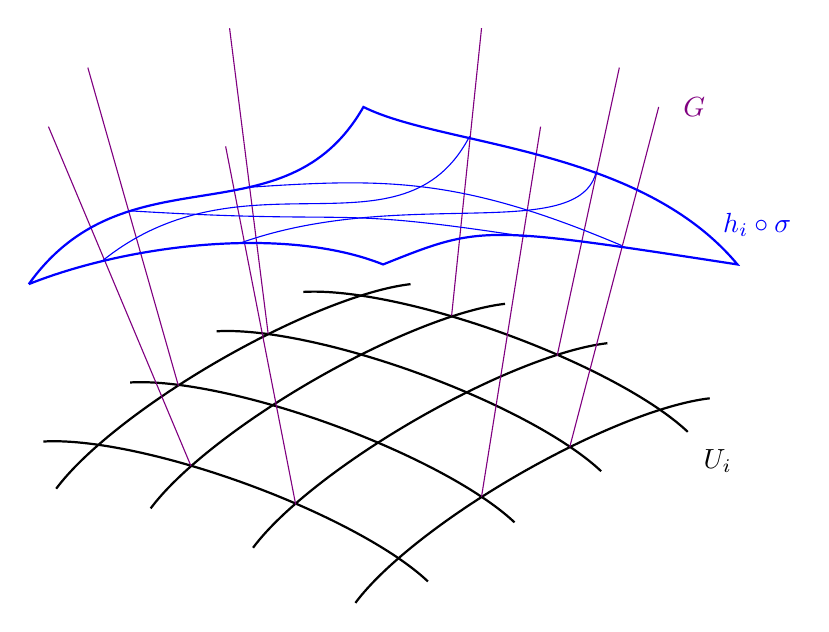
\begin{tikzpicture}%[scale=0.9]
	%\draw[opacity=0.1] (-4.5,-4.5) grid (4.5,4.5);

	%\draw (-1,-4)  .. controls (0,-2.5) and (1.5,-1.75) ..  (4,-2);

% BASE

	% gauche
	\draw[thick, xshift=1.3cm, yshift=-3.2cm, rotate=30]
		(3,0) arc [start angle=30, end angle =150, radius = 3, y radius = 0.75];
		
	\draw[thick, xshift=0cm, yshift=-2.5cm, rotate=30]
		(3,0) arc [start angle=30, end angle =150, radius = 3, y radius = 0.75];
		
	\draw[thick, xshift=-1.3cm, yshift=-2cm, rotate=30]
		(3,0) arc [start angle=30, end angle =150, radius = 3, y radius = 0.75];
		
	\draw[thick, xshift=-2.5cm, yshift=-1.75cm, rotate=30]
		(3,0) arc [start angle=30, end angle =150, radius = 3, y radius = 0.75];
		
	% droite
	\draw[thick, xshift=-2.5cm, yshift=-3cm, rotate=-20]
		(3,0) arc [start angle=30, end angle =150, radius = 3, y radius = 0.75];
	
	\draw[thick, xshift=-1.4cm, yshift=-2.25cm, rotate=-20]
		(3,0) arc [start angle=30, end angle =150, radius = 3, y radius = 0.75];
	
	\draw[thick, xshift=-0.3cm, yshift=-1.6cm, rotate=-20]
		(3,0) arc [start angle=30, end angle =150, radius = 3, y radius = 0.75];
	
	\draw[thick, xshift=0.8cm, yshift=-1.1cm, rotate=-20]
		(3,0) arc [start angle=30, end angle =150, radius = 3, y radius = 0.75];
	
	
% FIBRES

	\draw[violet] (-1.36,-3.05) -- (-2.25,1.5);
	\draw[violet] (1,-2.95) -- (1.75,1.75);
	
	\draw[violet] (-2.69,-2.56) -- (-4.5,1.75);
	\draw[violet] (2.12,-2.32) -- (3.25,2);
	
	\draw[violet] (-2.85,-1.54) -- (-4,2.5);
	\draw[violet] (1.96,-1.16) -- (2.75,2.5);
	
	\draw[violet] (-1.71,-0.88) -- (-2.2,3);
	\draw[violet] (0.62,-0.65) -- (1,3);
	
	
% SECTION

	%frame
	\draw[thick, blue] (-4.75,-0.25) .. controls (-3.5,1.5) and (-1.5,0.25) ..  
		(-0.5,2) .. controls (0.5,1.5) and (3,1.5) ..
		(4.25,0) .. controls (1,0.5) ..
		(-0.25,0) .. controls (-1.5,0.5) and (-3.5,0.25) ..
		(-4.75,-0.25);
		
	% coordo droite
	\draw[blue] (-3.45,0.68) .. controls (-0.5,0.5) and (-1,0.75) .. (1.58,0.35);
	\draw[blue] (-1.95,0.98) .. controls (-0.2,1.1) and (0.75,1.1) .. (2.78,0.24);
	
	%coordo gauche
	\draw[blue] (-3.81,0.05) .. controls (-2,1.5) and (0,0) .. (0.85,1.63);
	\draw[blue] (-2.04,0.28) .. controls (0,1) and (2.25,0.25) .. (2.46,1.19);
	
% NOTATION
	\draw (4,-2.5) node{ $U_i$};
	\draw (3.7,2) node{\color{violet} $G$};
	\draw (4.5,0.5) node{\color{blue} $h_i \circ \sigma$};
	
\end{tikzpicture}}
		
		\ffigbox{\caption[Représentation de la section canonique]
			{Représentation de la section canonique définie par rapport à $G$ avec une seconde section  $\sigma(x) = \sigma_i(x)\cdot g(x)$. Cette fois $B$ est une variété de dimension 1. % Sont également représentés leur espaces tangents horizontaux respectifs avec la transformation permettant de passer l'un à l'autre.
		}}{
			
\includegraphics[width=0.45\textwidth]{fig/placeholder}
			\label{fig:section_cano}}
	\end{floatrow}
\end{figure}
\noindent
Ensuite, les hypothèses sur $P(G,B)$ sont telles que $G$ agit transitivement et librement (ou sans point fixe) sur $P$. C'est-à-dire que, sur une même fibre, tout point peut être atteint par n'importe quel autre via l'action de $G$ (transitivité) :
\begin{align*}
	\forall x\in B,\quad \forall p,q\in P_x,\ \exists t(p,q)\in G\ |\ p = q\cdot t(p,q) 
\end{align*}
et que la seule façon de laisse les points invariants par cette même action est de passer par l'élément neutre $e$ (libre) :
\begin{align*}
	\forall (p,g)\in P\times G,\quad p = p\cdot g\ \Lr\ g=e
\end{align*}
\\
De la transitivité de $G$, découle le fait que toutes les sections locales $\sigma$ au dessus de $U_i$ peuvent s'écrire à partir d'une même section $\sigma_i$ via la formule :
\[\forall x\in B,\qquad \sigma(x) = \sigma_i(x) \cdot t\big(\sigma_i(x), \sigma(x)\big)\]
Son caractère libre, lui assure l'unicité d'un choix canonique de section $\sigma_i$ sur $U_i$. Elle est donnée par :
\[{h_i}(x,e) = \sigma_i(x)\]
Cela mène à la définition :
\begin{definition}[Fonctions de transitions]
	L'intersection de deux cartes  est noté $U_{ij} = U_i\cap U_j$ et le passage d'une section local canonique est donné par :
	\[\forall x\in U_{ij},\qquad \sigma_j(x) = \sigma_i(x) \cdot t\big(\sigma_i(x), \sigma_j(x)\big)\]
	L'élément de $G$, $t(\sigma_i, \sigma_j)$, est alors appelé \emph{fonction de transition} et sera noté $\varphi_{ij}$. Elle fait effectivement la transition entre deux cartes dans le sens où :
	\[\forall (g,x)\in G\times U_{ij},\qquad {h_i}^{-1} \circ h_j(g,x) = \big( \varphi_{ij}(x)g, x \big)\]
\end{definition}
\skipl




\subsubsection{Le fibré $\bf{\VFP}$}\label{subsec:SUPC_VFP}

Dans notre cas $\S{n}$ qui fait office d'espace totale avec $\PC{n}$ la base et $\U{1}$ pour le groupe structural.
\\
Pour obtenir la projection de $\S{n}$ sur $\PC{n}$, il suffit de prendre la restriction de $\pi$ à $\S{n}$. En tenant compte de la normalisation, les coordonnées locales sur $\PC{n}$ se réécrivent, $\forall w\in U_i$ :
\begin{align*}
	w^\mu = \frac{z^\mu}{z^i} &= \frac{z^\mu}{|z^i|e^{i\arg (z^i)}} = \frac{z^{\mu}}{\sqrt{1 - \sum_{\nu \neq i} |z^\nu|^2}} e^{-i\arg(z^i)}  &  \text{car }\quad \sum \big|z^\nu\big|^2 = \|z\|^2 = 1
\end{align*}
\\
On constate bien que $w^\mu$ n'est définie par rapport à $z^\mu$ qu'à un choix de phase $e^{-i\arg z^i}\in \U{1}$ près. À l'inverse, un représentant $z_i$ dans $\S{n}$ de $w\in U_i$ aura pour coefficient :
\begin{align*}
	\forall \mu\neq i,\quad {z_i}^\mu &= \frac{w^\mu}{\|w\|}e^{i\theta}  &  {z_i}^i &= \frac{1}{\|w\|}e^{i\theta} 
\end{align*}
\\
La norme de $w$ étant à comprendre au sens des coordonnées locales sur $U_i$\footnote{\itshape
	C'est un abus de notation, $w$ n'a pas de norme en ce sens là puisqu'elle dépend du choix de carte $U_i$. Mais ici tout le raisonnement est purement local, donc ce n'est pas un problème.
} :
\begin{align*}
	\|w\|^2 = \big\|(w^\mu)_{1\leq \mu\leq n}\big\|^2 = \frac{1}{|{z_i}^i|^2}\sum_{\nu \neq i} \big|{z_i}^\nu\big|^2 = \frac{1 - |{z_i}^i|^2}{|{z_i}^i|^2} &\Llr\ \big| {z_i}^i \big|^2 \|w\|^2 = 1 - \big|{z_i}^i\big|^2 \\
	&\Llr\ \big|{z_i}^i\big|^2 = \frac{1}{1 + \|w\|^2} \\
	&\Llr\ \big|{z_i}^i\big| = \frac{1}{\sqrt{1 + w^\nu \congu{w}_\nu}}
\end{align*}
D'où l'expression des coefficients de $z_i\in\S{n}$ :
\begin{align*}
	 \forall \mu\neq i,\quad {z_i}^\mu &= \frac{w^\mu}{\sqrt{1 + w^\nu \congu{w}_\nu}}e^{i\theta}  &  {z_i}^i &= \frac{1}{\sqrt{1 + w^\nu \congu{w}_\nu}}e^{i\theta} 
\end{align*}
\\

Tout cela permet d'écrire $\S{n}$ comme une variété fibrée principale :
\begin{proposition}
	La $(2n+1)-$sphère $\S{n}$, vu comme variété plongée dans $\C^n$ est une VFP de base $\PC{n}$ et de fibre type $\U{1}$. L'action de $\U{1}$ sur $\S{n}$ est induite par la multiplication par un scalaire complexe et où :
	\begin{itemize}
		\item La fibration $\pi$ est la projection canonique de $\S{n}$ sur $\PC{n}$ :
		\begin{equation}
			\pi\ :\ \begin{aligned} \S{n}\ &\lr\ \PC{n} \\ z\quad\ &\lmt\ \ [z]\end{aligned}
		\end{equation}
		
		\item Les cartes locales $h_i$ s'écrivent :
		\begin{equation}
			\forall w \in U_i,\ \forall e^{i\theta}\in\U{1},\  h_i(w,e^{i\theta}) = \frac{(w^0,\cdots, 1,\cdots, w^n)}{\sqrt{1 + w^\nu \congu{w}_\nu}}e^{i\theta} \in \S{n}
		\end{equation}
		
		\item Les sections canoniques $\sigma_i$ au dessus des $U_i$, elles,  sont définies par :
		\begin{equation}
			\forall w \in U_i,\ \sigma_i(w) = h_i(w, 1) = \frac{1}{\sqrt{1 + w^\nu \congu{w}_\nu}}(w^0,\cdots, 1,\cdots, w^n)
		\end{equation}
		
		\item Les fonctions de transitions entre deux cartes $U_i$ et $U_j$ s'écrivent :
		\begin{align}
			\varphi_{ij}(w) &= e^{-i \arg (z_i^i)} e^{i \arg (z_j^j)}  &  \text{ où }&\qquad z_{i,j} = \phi_{i,j}(w)
		\end{align}
	\end{itemize}
\end{proposition}
\skipl




\subsection{Espaces horizontaux et connexion}\label{subsec:connexion2VFP}

Le cadre étant posé, pour retrouver la notion de fréquence instantanée, il est nécessaire de munir $\VFP$ d'une connexion. Cette dernière est introduit comme suit.

\subsubsection{Définition général}\label{subsec:def2conn}

Comme $P$ ressemble localement à un produit $G\times U_i$, il est utile de séparer ses espaces tangents $\tg[p]{P}$ comme une somme directe d'espaces tangents respectivement aux fibres et à la base. Conformément aux représentations précédentes (\cref{fig:ruban2modius,fig:section_cano,fig:section_local}), les premiers sont appelées espaces tangents \emph{verticaux}, les seconds \emph{horizontaux} et l'on note :
\[\forall p\in P,\qquad \tg[p]{P} = \vg[p]{P} \oplus \hg[p]{P}\]
\\
Les tangents verticaux $\vg[p]{P}$ se définissent canoniquement via $\pi$, en tant que noyau de sa différentielle :
\[\vg[p]{P} \defeq \Ker (\tg[p]{\pi}) = \big\{ v\in\tg[p]{P}\ |\ \tg[p]{\pi}(v)=0 \big\}\]
\\ 
Ce n'est en revanche pas le cas des espaces horizontaux. Il faut donc faire un choix pour les $\hg[p]{P}$ et c'est ce choix qui est appelé \emph{connexion} (elle connecte les espace tangents entre eux).
Comme pour les vercticaux, ces sous-espaces peuvent être caractérisés par une 1-forme différentiable $\conn$ sur $P$ à valeur dans $\vg{P}$, auquel cas :
\[\forall p\in P,\quad \hg[p]{P} = \Ker(\conn_p)\]
\skipl

Dans le cas des VFP, une connexion doit en plus avoir de bonnes propriétés au regarde de l'action de $G$ sur $P$, aboutissant à la définition :

\begin{definition}[Connexion sur VFP] \label{def:connexion2VFP}
	Une \emph{connexion} sur une VFP $P(G,B)$ est la donnée d'un sous-espace tangent, $\hg[p]{P}\subset \tg[p]{P}$, en tout point de $p\in P$ tel que :
	\begin{itemize}
		
		\item $\hg{P}$ dépend différentiellement de $p$ (``dépendre différentiellement'' à un sens précis pour les sous-espaces mais qui ne sera pas utile pour la suite).
		
		\item $\hg[p]{P}$ est supplémentaire à $\vg[p]{P}$ dans $\tg[p]{P}$ :
		\begin{equation}\label{eq:TP=V+H}
			\tg[p]{P} = \vg[p]{P} \oplus \hg[p]{P}
		\end{equation}
		
		\item l'assignation des $\hg[p]{P}$ est invariante par l'action de $G$ au sens où :
		\begin{equation}\label{eq:conn_G-inv}
			\forall (p,g)\in P\times G,\quad \hg[R_g(p)]{P} = R_{g*} (\hg[p]{P}) = \big\{R_{g*}(\bf{v})\ |\ \bf{v} \in \hg[p]{P} \big\}
		\end{equation}
		Que l'on notera plus simplement (\cf annexe \ref{ann:2Lie}) :
		\begin{equation}
		\forall (p,g)\in P\times G,\quad \hg[p\cdot g]{P} = \hg[p]{P}\cdot g = \big\{\bf{v}\cdot g\ |\ \bf{v} \in \hg[p]{P} \big\}
		\end{equation}
	\end{itemize}
\end{definition}
\skipl

Au delà d'assurer une compatibilité entre $H$ et $G$, l'équation \eqref{eq:conn_G-inv} permet de n'avoir à définir la connexion qu'en un seul point de chaque fibre, les autres se déduisant par cette formule. 
Concrètement, pour tout point de la base $x\in U_i$, il suffit de la définir en $\sigma_i(x) = h_i(e, x)$, de sorte que l'espace horizontale en tout autre point $\ p=h_i(g, x) = \sigma_i(x)\cdot g$ au dessus de $x$ sera donné par :
\[\hg[p]{P} = \hg[\sigma_i(x)]{P}\cdot g\]
\\
Aussi, le fait que $G$ soit un groupe de Lie permet de lié son algèbre $\mathfrak{g}\cong \tg[e]{G}$ au tangent verticaux via l'application $\#$ : \footnote{\itshape 
	Les vecteurs tangents étant des formes linéaire, $A^\#(p)$ est plus précisément définie par l'application :
	\[A^\#(p) : f\ \lmt\  \frac{d}{dt} f\big( p\cdot \exp(tA) \big)\Big|_{t=0}\]}
\[\forall (p,A)\in P\times \mathfrak{g},\ \forall f\in\conti{P}{\R},\quad A^\#(p) = \frac{d}{dt} p\cdot \exp(tA) \Big|_{t=0}\in\vg[p]{P}\]
\\
Sachant cela, toujours dans le cas des VFP, la $1-$forme de connexion est à valeur dans $\mathfrak{g}$ :

\begin{definition}[$1-$forme de connexion] \label{def:1-form2conn}
	La \emph{$1-$forme de connexion} $\conn$ d'une VFP $P(G,B)$ est définie comme la 1-forme différentiable sur $P$ à valeur dans $\mathfrak{g}$ (\ie~en tout point $p\in P$, $\conn_p$ est à valeur de $\tg[p]{P}$ dans $\mathfrak{g}$), telle que $\forall p\in P$ :
	\begin{align} \label{eq:1-form2conn}
		\forall A\in \mathfrak{g},\ \conn_p\big(A^\#(p)\big) &= A  &  \hg[p]{P} &= \Ker(\conn_p)
	\end{align}
	\begin{equation} \label{eq:1-form_G-inv}
		\forall \bf{v}\in\tg[p]{P},\quad \conn_{p\cdot g}(\bf{v}\cdot g) \defeq \conn_{p\cdot g}(R_{g\, *}(\bf{v})) = g^{-1}\conn_p(\bf{v})g
	\end{equation}
	\skipl
	
	Tout comme les $H[p]{P}$, la troisième égalité assure que $\conn$ n'a besoin d'être définie que sur un point de chaque fibre. Cela permet de définir $\conn$ localement non pas sur $\ U_i\times G$, mais seulement sur $\ U_i \cong U_i \times \{e\}$. Ainsi, $\conn$ induit une 1-forme sur les cartes $U_i$ par l'image réciproque des sections canonique $\sigma_i$. Elles sont notées $\locconn_i \defeq \sigma_i^*\conn$ et sur le chevauchement $U_i\cap U_j$, elles vérifient :
	\begin{equation}\label{eq:conn_local}
		\locconn_j = {\varphi_{ij}}^{-1} \locconn_i \varphi_{ij} + {\varphi_{ij}}^{-1} d \varphi_{ij}
	\end{equation}
\end{definition}
\skipl


Munir $P(G,B)$ d'une connexion permet, entre autre de définir la notion de relèvement horizontal :
\begin{definition}[Relèvement horizontal]
	Étant donné une trajectoire $\ \rho : \R\ \lr B\ $ sur la base et un point $\gamma_0\in \rho(0)G$ au dessus de $\rho(0)$, il existe un unique relèvement $\gamma$ de $\rho$ donc les vecteurs tangents sont tous horizontaux. \ie~tel que $\forall t\in\R$ :
	\begin{align} \label{eq:condi2hori_lift}
	\pi\circ\gamma(t) &= \rho(t)  &  \dot{\gamma}(t) &\in \hg[\gamma(t)]{P} &  \gamma(0) &= \gamma_0
	\end{align}
	\\
	On parle de \emph{relèvement horizontal} (\emph{horizontal lift}, ou \emph{transport parallèle} de $\gamma_0$ le long de $\rho$) puisque $\gamma$ n'a pas de déplacement vertical au sens de la connexion. Du point de vue de la 1-forme $\omega$, si $\gamma$ s'écrit localement $\gamma_i = \sigma_i(\rho) g_i$, alors $g_i$ vérifie l'équation (d'où vient l'unicité du relèvement) :
	\begin{equation} \label{eq:EDP2hori_lift}
		\frac{d}{dt}g_i(t)  = - \locconn_i\rho(t) \cdot g_i(t)
	\end{equation}
	\\
	Si maintenant $\gamma$ est une trajectoire de $P$, on dira, par abus de langage, que $\Tilde{\gamma}$ est le relèvement horizontale de $\gamma$ si c'est le relèvement horizontale de sa projection $\pi\circ\gamma$ avec la condition initiale $\ \Tilde{\gamma}(0) = \gamma(0)$.
\end{definition}
\skipl

Pour la suite, il sera utile d'avoir l'expression d'une trajectoire $\gamma:\R\lr P$ par rapport à son relèvement horizontale $\Tilde{\gamma}$. Pour l'obtenir, on note  $\gamma = \Tilde{\gamma}\cdot g$, de sorte que sa dérivée s'écrive :
\[\dot{\gamma} = \dot{\Tilde{\gamma}}\cdot g + \Tilde{\gamma}\cdot dg = \dot{\Tilde{\gamma}}\cdot g + \gamma \cdot g^{-1}dg\]
\\
Ce à quoi on applique $\conn$, donnant :
\begin{align*}
	\conn_\gamma(\dot{\gamma}) &= \conn_\gamma\big( \dot{\Tilde{\gamma}}\cdot g \big) + \conn_\gamma \big( \gamma \cdot g^{-1}dg \big) \\
	&= g^{-1}\conn_{\Tilde{\gamma}}\big(\dot{\Tilde{\gamma}} \big) g + \conn_\gamma \big( \gamma \cdot g^{-1}dg \big)   &  &\text{d'après \eqref{eq:1-form_G-inv}} \\
	&= \conn_\gamma \big( \gamma \cdot g^{-1}dg \big)  &  &\text{car $\Tilde{\gamma}$ est horizontale}
\end{align*}
\\
Le terme $g^{-1}dg$ restant étant un vecteur de $\ g^{-1}\tg[g]{G}\cong \tg[e]{G}\cong \mathfrak{g}$ et :
\[\conn_\gamma(\dot{\gamma}) = \conn_\gamma \big( \gamma \cdot g^{-1}dg \big) = \conn_\gamma \big( (g^{-1}dg)^\#(p) \big) = g^{-1}dg\]
\\
D'où $\ \gamma = \Tilde{\gamma}\cdot g\ $ avec $g$ est solution de :
\begin{equation} \label{eq:deviation2hozi}
	\frac{d}{dt}g(t)  = g(t) \conn_{\gamma(t)}\big( \dot{\gamma}(t) \big)
\end{equation}
\skipl



\subsubsection{Choix de connexion sur $\bf{\VFP}$}\label{subsec:conn2SUPC}

Dans le cas de  $\VFP$, la métrique sur $\S{n}$ induit naturellement un choix de connexion car la projection $\pi$ est une submersion dite riemannienne \cite{kayban_riemannian_nodate}. Formellement, c'est dire que la projection de $\S{n}$ sur $\PC{n}$ est telle que :
\begin{equation} \label{eq:sub_riem}
	\forall p\in \pi^{-1}(w),\ \forall \bf{u},\bf{v}\in\tg[p]{\S{n}},\quad  g_{\pi(p)}\big( \pi_*\bf{u}, \pi_*\bf{v}\big) = \langle \bf{u}_H, \bf{v}_H\rangle
\end{equation}
\\
où $g$ est la partie réelle\footnote{\itshape
	Cette métrique induite ne peut pas être hermitienne car $\S{n}$ n'est pas une variété complexe.}
hermitienne de la métrique de Fubini-Study. Plus concrètement, les espaces tangents de $\S{n}$ s'écrivent :
\[\tg[p]{\S{n}} = \Vec\{p\}^\perp \defeq \big\{ \bf{v}\in\C^{n+1}\ |\  \Re e \langle \bf{v},p\rangle = 0\big\}\]
\\
et sachant que $ip\in \Vec\{p\}^\perp$, ils se séparent en deux composantes orthogonales :
\[\tg[p]{\S{n}} = \Vec\{p\}^\perp = \Vec\{ip\} \oplus \Vec\{ip\}^\perp\]
\\
Ainsi, la nature de $\pi$ \eqref{eq:sub_riem} est telle que le premier membre est l’espace tangent vertical à $p$ et le second invariant par l'action de $\U{1}$ :
\[\forall e^{i\theta}\in\U{1},\quad \Vec\big\{i(e^{i\theta}p)\big\}^\perp = \Vec\{ip\}^\perp\]
\\
Ce qui permet de poser $\ \hg[p]{\S{n}} \defeq \Vec\{ip\}^\perp\ $ et donne directement la 1-forme associée :
\[\begin{aligned}
	\hg[p]{\S{n}} &= \big\{\bf{v}\in\tg[p]{\S{n}}\ |\ \Re e \langle \bf{v}, ip \rangle = 0\} \\
	&= \big\{\bf{v}\in\tg[p]{\S{n}}\ |\ \Im m\langle \bf{v}, p \rangle = 0\}
\end{aligned}
\quad \Llr\quad \conn_p(\bf{v}) = \Im m\langle \bf{v},p\rangle\]
\\
Enfin, comme l'algèbre de Lie de $\U{1}$ est $\u{1}\cong i\R$, il convient de poser :
\begin{equation}\label{eq:conn2sub_riem}
	\forall p\in\S{n},\ \forall \bf{v}\in\tg[p]{\S{n}},\qquad \conn_p(\bf{v}) \defeq i\Im m\langle \bf{v},p\rangle
\end{equation}
\\
Un tel choix de connexion n'est pas anodin d'un point de vue signal puisque $\conn$ donne la fréquence instantanée telle que définie dans la \cref{part:param_instant} précédente et c'est la première chose qui sera justifier dans la partie suivante.
\\




\section{\wip Interprétation des trois phases dans ce cadre} \label{sec:phases_dans_VFP}

Résumons la situation. Pour étudier le comportement des fréquentielles d'un signal multivarié complexe, il est utile de voir l'espace de tel signaux, $\C^{n+1}$, comme le produit :
\[\C^{n+1} \cong \R^{+_*} \times \VFP\]
\\
Dans ce cadre, la variété $\VFP$ est naturellement -- par la projection $\pi$ -- munie d'une connexion qui, par ailleurs ressemble beaucoup à la formule de la fréquence instantanée \eqref{eq:phas_inst_v1} vue en première partie.
%La question est maintenant de savoir comment comprendre l'émergence de la phase géométrique dans ce cadre. Pour se faire, suivant les travaux de Aharonov et Anandan \cite[sec. 4, p. 53]{bohm_geometric_2003}
\\



\subsection{Fréquence instantanée et phase dynamique sur $\bf{\VFP}$}


Pour comprendre pourquoi le choix de connexion \eqref{eq:conn2sub_riem} est justifié du point de vue signal, on se propose de prendre le problème par l'autre bout : comment définir la notion de fréquence instantanée d'un signal dans la variété $\VFP$ ?
\\
 
Comme, à chaque instant $t$, un signal $\gamma$ sur $\S{n}$ est représenté par une pair $(e^{i\alpha(t)}, \rho(t))\in\U{1}\times\PC{n}$ à travers les $h_i$,  l'un serait tenté de voir $\alpha(t)$ comme la fréquence du signal et $\rho(t)$ comme l'état de polarisation.
\\
Le problème de cette représentation est qu'elle dépend du choix de carte $U_i$, ainsi sur l'intersection $U_{ij}$, $\gamma$ aurait (au moins) deux notions de fréquence instantanée.
\\

C'est là qu'intervient la connexion. D'une part, la 1-forme $\conn$ associée est définie globalement sur le fibré, autrement dit, elle est indépendante des représentations locales de $\gamma$.
\\
D'autre part, le relèvement horizontal $\Tilde{\gamma}$ d'une courbe $\rho\subset\PC{n}$, par définition, n'a pas de variation verticale. Dans notre cas, cela signifie que $\Tilde{\gamma}$ n'a pas de variation dans la direction de $\U{1}$, donc son état de polarisation (composante sur $\PC{n}$) varie mais pas ses ``fréquences''.
\\
Ainsi, le relèvement horizontale $\Tilde{\gamma}$ d'un signal $\gamma$ s'interprète comme une version de ce dernier $\gamma$ dénué de toute fréquence instantanée.
L'action $\alpha$ permettant de passé de $\Tilde{\gamma}(t)$ à $\gamma(t)$ (\ie~$(t) = e^{i\alpha(t)} \Tilde{\gamma}(t)$) peut alors être comprise comme la fréquence instantanée du signal (voir \cref{fig:freq_inst_geodiff,fig:horiz_lift_2var} ci-dessous)	
\\

\begin{remarque}
	Un signal qui n'aurait pas fréquence instantanée mais une polarisation instantanée n'a pas vraiment de sens. 
	Cela revoit à notre discussion de première partie : la fréquence instantanée d'un signal univarié devait contenir les hautes fréquences et son amplitude les basses.
	Ici le problème est le même, mais avec l'état de polarisation en lieu de l’amplitude. Pour s'en convaincre, il est utile de retourner sur le cas bivarié.
	\\
	La projection sur $\PC{2}$ de $\gamma$ représente l'ellipse de polarisation instantanée. 
	Mais si $\gamma$ n'as pas de fréquence instantanée, alors $\gamma(t)$ n'est plus représenté que par le sommet de l’ellipse paramétrée par $\rho_\gamma$. 
	L'on pourrait alors argumenter que tout signal peut être décrit par la seule variation de son état de polarisation, ce qui est parfaitement inintéressant.
	
	Cette vision du relèvement horizontale est donc purement formelle et, si elle à bien un sens géométrique, elle ne correspond à rien en terme de signal.
\end{remarque}
\skipl

\begin{figure}[H]
	\begin{floatrow}		
		\ffigbox{ \label{fig:freq_inst_geodiff}
			\caption[Interprétation géométrique de la fréquence instantanée]{Fréquence instantanée d'un signal $x$ vu comme variation vertical de $x$ par rapport à son relèvement horizontale $\Tilde{x}$ associé. À noter que $\Tilde{x}$ ne dépend pas des cartes mais dépend de la trajectoir $\rho_x$ de $x$ sur $\PC{n}$.}}
			{
\includegraphics[width=0.45\textwidth]{fig/placeholder}}
			
		\ffigbox{ \label{fig:horiz_lift_2var}
			\caption[Exemple relèvement horizontale]{Exemple du relèvement horizontale d'une signal bivarié}}
		{
\includegraphics[width=0.45\textwidth]{fig/placeholder}}
	\end{floatrow}
\end{figure}

En admettant l'interprétation de la 1-forme de connexion comme fréquence instantanée, les discussions de première partie (\Cref{subsec:intro_phased}) suggère de choisir :
\begin{equation} \label{eq:conn2SUPC}
	\forall x\in\S{n},\ \forall \bf{v}\in\tg[x]{\S{n}},\quad \conn_p(\bf{v}) = i\Im m \langle \bf{v}, x\rangle
\end{equation}
\\
La phase dynamique, s'interprète alors comme la déviation du signal à son par rapport à son relèvement horizontale. Ainsi, $\ g = e^{i\phased(\gamma)}\ $ est solution de \eqref{eq:deviation2hozi}, qui se réécrit alors :
\[\forall t\in\R,\quad \left\{ \begin{aligned}
	g'(t)  &= g(t)\, i\Im m \big\langle \dot{\gamma}(t) , \gamma(t) \big\rangle \\
	g(t_0) &= 1
\end{aligned}\ \right. \Llr\ g(t) = e^{\int_{t_0}^t i\Im m\langle \dot{\gamma}(s) , \gamma(s) \rangle ds}\]
\\
Ce qui redonne la formule :
\begin{equation}\label{eq:phased_vgeodiff}
	\phased(\gamma, t_0, t) = \int_{t_0}^t \Im m\big\langle \dot{\gamma}(s) , \gamma(s) \big\rangle ds
\end{equation}
\skipl

Chose importante tout de même : si cette définition de la phase dynamique est bien indépendante du choix de carte, elle dépend en revanche du relèvement horizontale de $\gamma$. Elle dépendant donc, \afortiori, de la trajectoire de la projection $\pi(\gamma)$ de $\gamma$ sur $\PC{n}$ et c'est de là que va émerger la phase géométrique.
\\



\subsection{Phase géométrique}


\subsubsection{\todo ... dans le cas pseudo-cyclique}

Comme dans la première partie de ce mémoire, pour mieux comprendre le comportement de la phase géométrique 

\begin{itemize}
	\item DEF : pseudo-cyclique
	
	\item Dans ce cas, la projection $C_\gamma$ de $\gamma$ sur $\PC{n}$ est (proprement) cyclique
	
	\item Comme, entre autre, Bohm l'explique dans \cite{bohm_geometric_2003}, en fonction du choix de relèvement on peut isoler les différentes phases de $\gamma$. 
	
	\item En particulier, $C_\gamma$ est cyclique, $\gamma(1)$ est dans la même fibre que $\gamma(0)$ et les trois se décrivent dans une même fibre $\gamma(0)\U{1} = \gamma(1)\U{1}$ :
	
	\item Étant donné le choix de connexion, le relèvement horizontale $\Tilde{\gamma}$ de $C_\gamma$ (à partir du point initiale $\gamma(0)$) n'a pas de phase dynamique. $\phased$ est donc donnée par différence de phase entre $\gamma(1)$ et $\Tilde{\gamma}(1)$
	
	\item Pour obtenir la phase géométrique, on considère une troisième relèvement, $\eta$, de $C_\gamma$ qui cette fois est proprement cyclique. Comme il n'a, par construction, par de phase totale, sa phase géométrique est égale à sa phase dynamique au signe près.
	
	\item Or, la phase $\phased(\eta)$ est, comme pour $\gamma$ donné par la différence de jauge entre $\Tilde{\gamma}(1)$ et $\eta(1)$.
	
	\item Tout cela est résumé par la \Cref{fig:phases_p-cycl} ci-dessous :
	\begin{figure}[h]
		
\includegraphics[width=0.4\textwidth]{fig/placeholder}
		\caption[Représentation des trois phases de $\gamma$ dans le cas pseudo-cyclique]{Représentation des trois phases de $\gamma$ dans le cas pseudo-cyclique.}
		\label{fig:phases_p-cycl}
	\end{figure}
	
	\item Remarque importante : le choix de relèvement cyclique $\eta$ n'est pas unique mais n'est pas important pour autant, puisque c'est la seule propriété $\eta(0)=\eta(1)$ qui permet d'avoir l'interprétation exposé juste avant. Cela traduit, par ailleurs, l'aspect invariant par transformation de jauge de $\phaseg$.
	
	\item Ce que cette représentation montre c'est que $\phaseg$ est donné par l'holonomie du trajet $\gamma$.
	
	\item DEF : holonomie
	
		
	
	\item Dans notre cas, la variété est connexe ce qui assure que $\Hol$ est un sous-groupe de Lie connexe du groupe structural, à savoir $\U{1}$. Ainsi, $\Hol = \U{1}$, ce qui montre que la phase géométrique peut prendre n'importe qu'elle valeur.
	
	\item Cette formulation est très jolie mais finalement que très peu instructive. 
	
	\item Rq : On pourrait alors se demander si $\phaseg$ ne pourrait pas, comme $\phased$, s'écrire comme l'intégrale d'une 1-forme sur $\PC{n}$.
	\\
	A cela, Mukunda \& Simon explique dans \cite{mukunda_quantum_1993} que non. Moralement, l'écriture $\phaseg = \phaset - \phased$ suggère que ça ne peut pas être le cas puisque la phase totale ne peut pas s'écrire comme l'intégrale d'une 1-forme.
	\\
	
	 Cela vient du fait que $\phaset$ est indépendant de la trajectoire de $\gamma$ sur $]0,1[$. Au mieux, elle peut être vu comme la longueur de la géodésique $\gamma_g$ sur $\S{n}$ entre les points $\gamma(0)$ et $\gamma(1)$. C'est-à-dire comme l'intégrale de la norme sur $\S{n}$ de $\dot{\gamma}_g$ le long de $\gamma_g$. Mais rien par rapport à $\gamma$
	
\end{itemize}




\subsection{\todo ... dans le cas général}

\begin{itemize}
	
	\item Si maintenant $\gamma$ est qu'elle conque, pour retrouver les interprétation précédente, le plus simple est encore de se ramener au cas pseudo-cyclique.
	
	\item Cela demande de refermer $\gamma$ de sorte à ne pas engendré plus de phase géométrique. En somme, on veut savoir qu'elles sont les trajectoire de $\S{n}$ qui n'engendre pas de phase géométrique.
	
	\item pour cela on étudie les géodésiques !
	
	\item Sachant le représentaiton par Stokes c'est plutôt simple : 
\end{itemize}




\subsection{\todo ... sur $\PC{n}$}

\begin{itemize}
	
	\item Cela étant dit, dans le cas cyclique $\phaseg$ et $\phased$ se confonde et cette propriété peut être exploitée.
	
	\item En effet, modulo l'exponentielle, la phase dynamique est l'intégrale de la connexion sur la courbe. Ainsi, d'après le théorme de Stokes, on a relation :
	\[\oint_\rho \locconn_i(d\rho) = \iint_\Sigma d\locconn_i(dx,dy) dx\,dy\]
	
	\item En effet,  la commutativité de $\U{1}$ fait que $\Hol$ est indépendant du relèvement $\eta(0)$ de $C_\gamma(0)$ 
	
	\item Ajouter à cela le fait que la connexion s'exprime exclusivement dans les cartes $U_i$, on se ramène à calcul un calcul de la phase géométrique exclusivement dans $\PC{n}$.
	
	\item Dans ce cas, la phase géométrique est l'intégrale sur un lacet d'une 1-forme et le théorème de Stokes peut s'appliquer :
	
	\item THEO de Stokes
	
	\item Dans notre cas : on obtient l’intégrale d'une forme symplectique sur l'aire entouré par le lacet $C_\gamma$ (je suspecte que ce soit $-i\Im m$(métrique F-S + à affiner) 
	
	\item En somme, cela se ramène à un calcul d'aire sur $\PC{n}$
	
	\item \thoughts{Un mot sur le lien avec Fisher}
	
\end{itemize}




%%%% ANNEXES %%%%



\begin{annexe}

\section{Annexe}

\subsection{\wip Variété différentielle complexe }\label{ann:VDC}

\textit{Pour plus de détails, voir \cite{nakahara_geometry_2003, ballmann_lectures_2006}.}
\\

$\manu$ sera une \emph{variété différentielle complexe} si elle satisfait les propriétés ci-dessus où $\R^n$ est remplacé par $\C^n$ et où la condition de difféomorphisme est remplacé par la condition d'holomorphisme. 
\\
Une application $f : \C^n\lr \C^n$ étant holomorphe si chacune de ses composantes vérifie l'équation de Cauchy-Riemann :
\[\forall x,y\in\R^n,\ \forall \mu,\qquad \frac{\partial f }{\partial y^\mu}(x+iy) = i \frac{\partial f }{\partial x^\mu}(x+iy)\]
\\
Les fonctions holomorphes étant automatiquement $C^\infty$, les variétés différentielles complexes sont toujours lisse, c'est-à-dire $C^\infty$. Aussi, $\manu$ est dite de dimension complexe $n$ et dimension (réel) $2n$, notés :
\begin{align}\label{eq:manuC-base_cano}
	\dim[\C](\manu) &\defeq n  &  \dim[\R] (\manu) \defeq \dim (\manu) = 2n
\end{align}
\\

Ensuite, pour le dire rapidement, la structure complexe de $\manu$ permet de séparer les espaces tangents en deux sous espaces. Pour ce faire, on commence par noter qu'en tout point $p\in\manu$ de coordonnée $z^\nu=x^\nu+iy^\nu$, l'espace tangent $\tg[p]{\manu}$, vu comme variété réelle, admet une base :
\begin{equation}
	\tg[p]{\manu} = \vec \left\{ \frac{\partial}{\partial x^1}, \cdots, \frac{\partial}{\partial x^n}, \frac{\partial}{\partial y^1}, \cdots,  \frac{\partial}{\partial y^n} \right\}
\end{equation}
\\
Plus tôt que de se basé sur les $x^\mu$ et $y^\mu$ pour séparer les $\tg[p]{\manu}$, on définit sur ces derniers un tenseur $J_p$ de type (1,1) tel que :
\begin{align}
	J_p \frac{\partial}{\partial x^\mu} &= \frac{\partial}{\partial y^\mu}  &  J_p \frac{\partial}{\partial y^\mu} &= -\frac{\partial}{\partial x^\mu}
\end{align}
\\
Ce tenseur est l'équivalent de la multiplication par $\pm i$ et le fait que $\manu$ soit complexe assure qu'il soit défini globalement, \ie~sur $\tg{\manu}$. Il est diagonaliseable dans la base :
\begin{align}\label{eq:manuC-base_holo}
	\partial_\mu = \frac{\partial}{\partial z^\mu} &\defeq \frac{1}{2}\left( \frac{\partial}{\partial x^\mu} - i\frac{\partial}{\partial y^\mu} \right)  
	&  
	\partial_{\bar{\mu}} = \frac{\partial}{\partial \overline{z}^\mu} &\defeq \frac{1}{2}\left( \frac{\partial}{\partial x^\mu} + i\frac{\partial}{\partial y^\mu} \right)
\end{align}
\\
Ainsi en fonction de la base (\eqref{eq:manuC-base_cano} ou \eqref{eq:manuC-base_holo}), $J_p$ va s'écrire :
\begin{align}
	J_p &= \begin{pmatrix}
		\text{\large\ 0\ }\Big. & I_n \\ -I_n & \text{\large\ 0\ }\Big.
	\end{pmatrix}  &
	J_p &= \begin{pmatrix}
		iI_n & \text{\large\ 0\ }\Big. \\ \text{\large\ 0\ }\Big. & -iI_n
	\end{pmatrix} 
\end{align}
\\
Finalement, $\tg{\manu}$ peut être séparé en deux sous-espaces engendré respectivement par les $\partial_\mu$ et $\partial_{\bar{\nu}}$. On parle de vecteur holomorphe et anti-holomorphe et on note :
\begin{align}
	\tg[p]{\manu}^+ &= \Vec\big\{ \partial_\mu\ |\ 1\leq \mu\leq n \big\}  &  \tg[p]{\manu}^- &= \Vec\big\{ \partial_{\bar{\mu}}\ |\ 1\leq \mu\leq n \big\}
\end{align}
\\ \\

forme kahlerienne :
\begin{equation}
	\Omega = g_{\mu \congu{\alpha}} {J^{\congu{\alpha}}}_{\congu{\nu}} dw^\mu \wedge d\congu{w}^\nu
\end{equation}
sur $\PC{n}$ :
\[\Omega(w) = i\frac{(1+w^\alpha \congu{w}_\alpha)\delta_{\mu\nu} - w_\mu \congu{w}_\nu}{(1+w^\alpha \congu{w}_\alpha)^2} dw^\mu \wedge d\congu{w}^\nu\]
\skipl



\subsection{\wip Dérivée extérieure de la connexion}

Par définition, sur l'ouvert $U_i$, la 1-forme de connexion local est définie par :
\[\locconn_i = {\sigma_i}^*\conn = \conn\circ \sigma_{i*}\]
\\
Soit, $\forall w\in U_i,\ \forall X\in\tg[w]{\PC{n}}$ :
\[\locconn_i(w)X= i\Im m \big\langle \sigma_{i*}(X), \sigma_i(w) \big\rangle\]
\\
où les $\sigma_{i*}$ s'écrivent, $\forall \mu$ :
\begin{align*}
	\mu &\neq i : &  \sigma_i(w)^\mu = \frac{w^\mu}{\sqrt{1 + w^\alpha\congu{w}_\alpha}}\quad \Lr\quad
	\sigma_{i*}(w)^\mu &= \frac{dw^\mu}{\sqrt{1 + w^\alpha\congu{w}_\alpha}} - \frac{w^\mu}{2(1 + w^\alpha\congu{w}_\alpha)^{\nicefrac{3}{2}}}2\Re e(w^\alpha d\congu{w}_\alpha) \\
	&  &  &= \frac{1}{\sqrt{1 + w^\alpha\congu{w}_\alpha}}\left(dw^\mu - w^\mu \frac{\Re e(w^\alpha d\congu{w}_\alpha)}{1 + w^\alpha\congu{w}_\alpha}\ \right)
	\\ \\
	\mu &= i :  &  \sigma_i(w)^\mu = \frac{1}{\sqrt{1 + w^\alpha\congu{w}_\alpha}}\quad \Lr\quad
	\sigma_{i*}(w)^\mu &= - \frac{\Re e(w^\alpha d\congu{w}_\alpha)}{(1 + w^\alpha\congu{w}_\alpha)^{\nicefrac{3}{2}}}
\end{align*}
\\
Ce qui donne\footnote{\itshape
	Dans le formule ci-dessous, les 0 et 1 sont placés à la $i^{eme}$ coordonnées.
} :
\begin{align*}
	\locconn_i(w) &= i\Im m \big\langle \sigma_{i*}(w), \sigma_i(w) \big\rangle \\
	&= i\Im m \left\langle \frac{1}{\sqrt{1 + w^\alpha\congu{w}_\alpha}}\left((dw^0,\cdots , 0, \cdots, dw^n) - (w^0,\cdots , 1, \cdots, w^n) \frac{\Re e(w^\alpha d\congu{w}_\alpha)}{1 + w^\alpha\congu{w}_\alpha}\ \right), \frac{(w^0,\cdots , 1, \cdots, w^n)}{\sqrt{1 + w^\alpha\congu{w}_\alpha}} \right\rangle \\
	&= \frac{1}{1 + w^\alpha\congu{w}_\alpha} i\Im m \left( \Big\langle (dw^0,\cdots , 0, \cdots, dw^n), (w^0,\cdots , 1, \cdots, w^n) \Big\rangle \bigg. \right. \\
	&\qquad\qquad\qquad\qquad\qquad - \left.  \frac{\Re e(w^\alpha d\congu{w}_\alpha)}{1 + w^\alpha\congu{w}_\alpha}\Big\langle (w^0,\cdots , 1, \cdots, w^n) , (w^0,\cdots , 1, \cdots, w^n) \Big\rangle \right) \\
	&= \frac{1}{1 + w^\alpha\congu{w}_\alpha} i\Im m \left( dw^\mu\congu{w}_\mu -  \frac{\Re e(w^\alpha d\congu{w}_\alpha)}{1 + w^\alpha\congu{w}_\alpha}\big( w^\nu\congu{w}_\nu +1 \big) \right)
\end{align*}
\\
Enfin, sachant que le second membre dans la partie imaginaire est réel, il vient :
\begin{align*}
	\locconn_i(w) = \frac{1}{1 + w^\alpha\congu{w}_\alpha} i\Im m \left( dw^\mu\congu{w}_\mu -  \frac{\Re e(w^\alpha d\congu{w}_\alpha)}{1 + w^\alpha\congu{w}_\alpha}\big( w^\nu\congu{w}_\nu +1 \big) \right) 
	&= \frac{1}{1 + w^\alpha\congu{w}_\alpha} i\Im m \big( dw^\mu\congu{w}_\mu \big) \\
	&= \frac{1}{1 + w^\alpha\congu{w}_\alpha} \frac{dw^\mu\congu{w}_\mu -  d\congu{w}^\nu w_\nu }{2}
\end{align*}
\\

Point de subtilité : les coefficients associées au $dw^\mu$ et $d\congu{w}^\nu$ doivent être traité séparément


\subsection{Géodésique de $\bf{\PC{n}}$}


\subsubsection{Métrique relevée dans les espaces horizontaux}


D'abord les vecteurs tangent de $\S{n}$ sont séparés en composantes verticale et horizontales :
\begin{align}
	\forall \bf{v}\in \tg[p]{\S{n}},\quad \bf{v} = \bf{v}_H + \omega_p(\bf{v})^\# &= \bf{v}_H + \frac{d}{dt}p\cdot \exp\big(it\Im m \langle \bf{v}, p \rangle\big)\Big|_{t=0} \\
	&= \bf{v}_H  + i\Im m \langle \bf{v}, p \rangle p
\end{align}
\\
Ainsi, $\forall \bf{u},\bf{v}\in \tg[p]{\S{n}}$ :
\begin{align*}
	g_{\pi(p)}( \pi_*\bf{u}, \pi_*\bf{v}) = \big\langle \bf{u}_H, \bf{v}_H \big\rangle &= \big\langle\bf{u} - \conn_p(\bf{u})^\#, \bf{v} - \conn_p(\bf{v})^\# \big\rangle \\
	&= \big\langle\bf{u}, \bf{v} \big\rangle  - \big\langle\bf{u}, \conn_p(\bf{v})^\# \big\rangle - \big\langle \conn_p(\bf{u})^\#, \bf{v} \big\rangle + \big\langle \conn_p(\bf{u})^\#, \conn_p(\bf{v})^\# \big\rangle \\
	&= \big\langle\bf{u}, \bf{v} \big\rangle  - \big\langle\bf{u},  i\Im m \langle \bf{v}, p \rangle p \big\rangle - \big\langle  i\Im m \langle \bf{u}, p \rangle p, \bf{v} \big\rangle + \big\langle  i\Im m \langle \bf{u}, p \rangle p,  i\Im m \langle \bf{v}, p \rangle p \big\rangle \\
	&= \big\langle\bf{u}, \bf{v} \big\rangle  + i\Im m \langle \bf{v}, p \rangle\big\langle\bf{u}, p \big\rangle - i\Im m \langle \bf{u}, p \rangle\big\langle p, \bf{v} \big\rangle - i\Im m \langle \bf{u}, p \rangle i\Im m \langle \bf{v}, p \rangle \big\langle p, p \big\rangle
\end{align*}
\\
Sachant que $\ \|p\|=1\ $ et $\ \Re e \langle \bf{v},p\rangle = 0$, il vient :
\begin{align*}
g_{\pi(p)}( \pi_*\bf{u}, \pi_*\bf{v}) 
	&= \big\langle\bf{u}, \bf{v} \big\rangle  + i\Im m \langle \bf{v}, p \rangle\big\langle\bf{u}, p \big\rangle - i\Im m \langle \bf{u}, p \rangle\big\langle p, \bf{v} \big\rangle - i\Im m \langle \bf{u}, p \rangle i\Im m \langle \bf{v}, p \rangle \big\langle p, p \big\rangle \\
	&= \big\langle\bf{u}, \bf{v} \big\rangle  -\Im m \langle \bf{v}, p \rangle \Im m\big\langle\bf{u}, p \big\rangle + \Im m \langle \bf{u}, p \rangle \Im m \big\langle p, \bf{v} \big\rangle - \langle \bf{u}, p \rangle \langle \bf{v}, p \rangle\\
	&= \big\langle\bf{u}, \bf{v} \big\rangle -  \langle \bf{u}, p \rangle \langle \bf{v}, p \rangle
\end{align*}

Ce qui donne en coordonnées locales sur $\S{n}$ : 
\[g = \delta_{\mu \nu} dz^\mu d\congu{z}^\nu - \delta_{\mu \beta}z^\mu d\congu{z}^\beta \delta_{\alpha \nu} dz^\alpha \congu{z}^\nu = \big( \delta_{\mu \nu} - z_\nu \congu{z}_\mu \big) dz^\mu d\congu{z}^\nu\]
\skipl



\subsubsection{Ecriture des géodésiques}

\textit{Les calculs de cette section reprenne en partie les calculs de Mukunda \& Simon \cite[sec. 4, p. 219]{mukunda_quantum_1993}.}
\\

Etant donnée, sur une variété $\manu$, une métrique $g$ de symbole de Christoffel associé $\Gamma$, une géodésique $\gamma$ de $\manu$ vérifie \cite{do_carmo_riemannian_1992} :
\begin{equation}\label{eq:EDP2geode}
	\forall \sigma,\quad \ddot{\gamma}^\sigma + \Gamma^\sigma _{\mu \nu} \dot{\gamma}^\mu \dot{\gamma}^\nu = 0
\end{equation}
\\
Pour une variété complexe, les contraintes apportés par les composantes holomorphe  et anti-holomorphe  sont les mêmes. Le système reste donc le même à la différence près que cette fois les symboles de Christoffel vont s'écrire\footnote{\itshape
	Les symétries imposées à $g$ par la forme symplectique $J$ annule la majorité des composantes de $g$ et \afortiori, de $\Gamma$. Voir \cite[sec. 8.4.3]{nakahara_geometry_2003}
} :
\begin{align}\label{eq:symb2Christo}
	\Gamma^\sigma _{\mu \alpha} &= g^{\sigma \congu{\beta}} \partial_{\mu} (g_{\alpha \congu{\beta}})  &  \Gamma^{\congu{\sigma}} _{\congu{\nu \beta}} &= g^{\alpha \congu{\sigma}} \partial_{\congu{\nu}} (g_{\alpha \congu{\beta}}) 
\end{align}
\\
Le système d'EDP \eqref{eq:EDP2geode} s'écrit alors :
\begin{align*}
	\ddot{\gamma}^\sigma + \Gamma^\sigma _{\mu \alpha}\,  \dot{\gamma}^\mu\, \dot{\gamma}^\alpha = 0 
	\quad &\Llr\quad
	\ddot{\gamma}^\sigma + g^{\sigma \congu{\beta}} \partial_{\mu} (g_{\alpha \congu{\beta}}) \, \dot{\gamma}^\mu\, \dot{\gamma}^\alpha = 0 \\
	&\Llr\quad 
	g_{\sigma \congu{\beta}}\, \ddot{\gamma}^\sigma + g_{\sigma \congu{\beta}}\, g^{\sigma \congu{\beta}} \partial_{\mu} (g_{\alpha \congu{\beta}}) \, \dot{\gamma}^\mu\, \dot{\gamma}^\alpha = 0 \\
	&\Llr\quad 
	g_{\sigma \congu{\beta}}\, \ddot{\gamma}^\sigma + \partial_{\mu} (g_{\alpha \congu{\beta}}) \, \dot{\gamma}^\mu\, \dot{\gamma}^\alpha = 0
\end{align*}
\\
Dans le cas de $\VFP$, les $\partial g_{\alpha \congu{\beta}}$ s'écrivent :
\begin{align*}
	\partial_{\mu} (g_{\alpha \congu{\beta}}) &= \partial_{\mu} \big( \delta_{\alpha \beta} - \congu{z}_\alpha z_\beta \big) = - \delta_{\mu\beta} \congu{z}_\alpha   &  
	\partial_{\congu{\nu}} (g_{\alpha \congu{\beta}}) &= \partial_{\congu{\nu}} \big( \delta_{\alpha \beta} - \congu{z}_\alpha z_\beta \big) = - \delta_{\nu \alpha} z_\beta
\end{align*}
\\
Donnant les équations :
\begin{align*}
	\forall \beta,\quad \begin{aligned}
		0 &= g_{\sigma \congu{\beta}}\, \ddot{\gamma}^\sigma + \partial_{\mu} (g_{\alpha \congu{\beta}}) \, \dot{\gamma}^\mu\, \dot{\gamma}^\alpha \\
		&= \big( \delta_{\sigma \beta} - \congu{\gamma}_\sigma \gamma_\beta \big)\, \ddot{\gamma}^\sigma - \delta_{\mu\beta} \congu{\gamma}_\alpha \, \dot{\gamma}^\mu\, \dot{\gamma}^\alpha \\
		&= \ddot{\gamma}_\beta - \gamma_\beta \langle \ddot{\gamma},\gamma\rangle - \dot{\gamma}_\beta \langle  \dot{\gamma}, \gamma \rangle 
	\end{aligned} \qquad \Llr\quad 
	0 = \ddot{\gamma} -  \langle \ddot{\gamma},\gamma\rangle \gamma -  \langle  \dot{\gamma}, \gamma \rangle \dot{\gamma}
\end{align*}
\\
Où l'équivalence est justifiée par le fait que les composantes anti-holomorphes des $\gamma, \dot{\gamma}, \ddot{\gamma}$ suivent les mêmes contraintes (à conjugaison près) celles holomorphes.

Pour résoudre ce système, le produit hermitien de ce dernier avec $\gamma$ est calculé :
\begin{align*}
	 \ddot{\gamma} =  \langle \ddot{\gamma},\gamma\rangle \gamma + \langle  \dot{\gamma}, \gamma \rangle \dot{\gamma} \quad 
	 &\Lr\quad \langle \ddot{\gamma}, \gamma \rangle =  \langle \ddot{\gamma},\gamma\rangle \langle \gamma, \gamma \rangle + \langle  \dot{\gamma}, \gamma \rangle^2 \\
	 &\Lr\quad 0 =  \langle  \dot{\gamma}, \gamma \rangle
\end{align*}
On retrouve alors le fait que $\dot{\gamma}$ est horizontale et $\ \ddot{\gamma} = \gamma \langle \ddot{\gamma},\gamma\rangle$.
\\
En appliquant à nouveau le produit hermitien mais de l'autre côté, cette fois :
\[\ddot{\gamma} = \gamma \langle \ddot{\gamma},\gamma\rangle\quad 
\Lr\quad \langle \gamma, \ddot{\gamma} \rangle = \langle  \gamma, \gamma \rangle \langle \ddot{\gamma},\gamma\rangle  =  \langle  \ddot{\gamma}, \gamma \rangle\]
\\
Sachant que $\gamma\in\S{n}$, on a alors :
\begin{align*}
	\|\gamma\| = 1\ &\Lr\ \langle \gamma, \dot{\gamma} \rangle + \langle \dot{\gamma}, \gamma \rangle =0 \\
	&\Lr\ \langle \gamma, \ddot{\gamma} \rangle + 2\langle \dot{\gamma}, \dot{\gamma} \rangle + \langle \ddot{\gamma}, \gamma \rangle =0 \\
	&\Lr\ \langle \gamma, \ddot{\gamma} \rangle = - \langle \dot{\gamma}, \dot{\gamma} \rangle
\end{align*}
\\
Finalement l'EDP devient :
\[\ddot{\gamma} = - \langle \dot{\gamma}, \dot{\gamma} \rangle \gamma \]
\\
Or, il existe une paramétrisation de $\gamma$ telle que $\|\gamma\| = 1$. D'où les solutions :
\[\gamma(t) = \gamma(t_0) \cos (t - t_0) + \dot{\gamma}(t_0) \sin (t - t_0)\]





%\subsection{Algèbre et groupe de Lie} \label{ann:2Lie}

%\subsubsection{Quelques généraliés}

%\subsubsection{Cas particulier : $\bf{\U{1}}$}





\end{annexe}




